\documentclass[tikz, border=2pt]{standalone}
\usepackage{amsmath}

\begin{document}
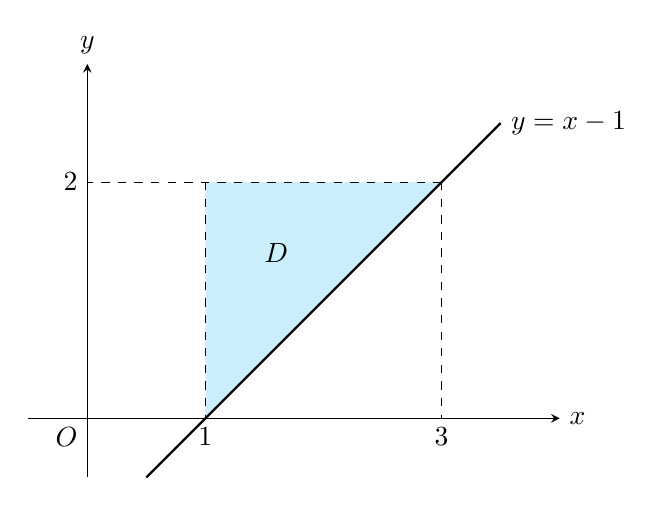
\begin{tikzpicture}[scale=1.5, >=stealth]
    % 填充积分区域 D (三角形：顶点为 (1,0), (3,2), (1,2))
    \fill[cyan!20] (1,0) -- (3,2) -- (1,2) -- cycle;

    % 画坐标轴
    \draw[->] (-0.5, 0) -- (4.0, 0) node[right] {$x$};
    \draw[->] (0, -0.5) -- (0, 3.0) node[above] {$y$};

    % 画直线 y = x - 1
    % 为了美观，线条稍微画长一点
    \draw[thick] (0.5, -0.5) -- (3.5, 2.5) node[right] {$y=x-1$};

    % 画边界辅助线
    \draw[dashed] (1,2) -- (1,0) node[below] {$1$};
    \draw[dashed] (3,2) -- (3,0) node[below] {$3$};
    \draw[dashed] (3,2) -- (0,2) node[left] {$2$};

    % 标注区域 D 和原点
    \node at (1.6, 1.4) {$D$};
    \node[below left] at (0,0) {$O$};
\end{tikzpicture}
\end{document}
